\documentclass[12pt]{article}
\usepackage[margin=1in]{geometry}
\usepackage[utf8]{inputenc}
\usepackage[spanish]{babel}
\usepackage{parskip}
\usepackage{setspace}
\usepackage{amsmath, amssymb}
\usepackage{graphicx}
\usepackage{hyperref} % Siempre debe ir al final.

% Opciones de Paquetes.
\decimalpoint           % {babel}
\onehalfspacing         % {setspace}
\graphicspath{{./img/}} % {graphicx}

% Encabezado.
\title{Sucesiones: Repaso.}
\author{MIT 18.01: Single Variable Calculus.}
\date{}


\begin{document}

\maketitle

\begin{abstract}
\noindent Para estudiar \textbf{series infinitas} se debe tener un conocimiento previo sobre las \textbf{sucesiones}. A continuación se hará una revisión de este concepto y algunas de sus propiedades usando como base los libros de Stewart\footnote{Stewart, James. "Sucesiones". En \textit{Cálculo. Trascendentes Tempranas}, 694-703. México: Cengage Learning Editores, 2017.} y Thomas\footnote{Thomas, George. "Sucesiones". En \textit{Cálculo. Una variable}, 532-41. México: Pearson Educación, 2010.}.
\end{abstract}


\section{Sucesiones.}

\subsection{Definición y características.}

Una \textbf{sucesión} (\textit{sequence} en inglés) es una \textbf{lista de números ordenados}. Un ejemplo es el siguiente:
\[
  a_{1}, \ a_{2}, \ a_{3}, \ \ldots, \ a_{n}, \ \ldots
\]
Cada número $a_{i}$, para $i = 1, \ \ldots, \ n, \ \ldots$, recibe el nombre de \textbf{término de la sucesión} y el orden está dado por el índice $i$.

\begin{table}[hbt!]
\centering

\begin{tabular}{c c c}
\hline
Índice & Término & Nombre \\
\hline
$1$ & $a_{1}$ & Primer término \\
$2$ & $a_{2}$ & Segundo término \\
$\vdots$ & $\vdots$ & $\vdots$ \\
$n$ & $a_{n}$ & $n$-ésimo término \\
$\vdots$ & $\vdots$ & $\vdots$ \\
\hline
\end{tabular}

\end{table}

Siempre se debe tener en consideración el \textbf{orden} de los términos en una sucesión. Por ejemplo,
\[
  \{2, \ 3, \ 5, \ 7\} \neq \{3, \ 2, \ 7, \ 5\}
\]
Ambas listas son sucesiones, pero no son iguales porque sus términos siguen un orden distinto.

Las sucesiones se suelen abreviar de dos maneras. Por ejemplo, $\{a_{1}, \ a_{2}, \ \ldots \}$ se puede denotar como:
\[
  \{a_{i}\} \qquad \text{o} \qquad \{a_{i}\}_{i = 1}^{\infty}
\]
Ambas se usan de manera intercambiada.

Es posible entender una sucesión como una \textbf{función}. Veamos la siguiente tabla.

\begin{table}[hbt!]
\centering

\begin{tabular}{c|c c c c}
$i$ & $1$ & $2$ & $3$ & $4$ \\
\hline
$\{a_{i}\}$ & $1/2$ & $1/3$ & $1/4$ & $1/5$
\end{tabular}

\end{table}

Como se aprecia en la tabla, cada término de $\{a_{i}\}_{i = 1}^{4}$ es la imagen única de su correspondiente índice $i$, donde $i \in \mathbb{Z}_{0}^{+}$ (i.e, incluye al cero). Por otra parte, los $a_{i}$ se encuentran en cualquier conjunto numérico. Así, es posible señalar que:
\[
  \{a_{i}\}: \mathbb{Z}_{0}^{+} \to X
\]
donde $X$ es un conjunto numérico cualquiera.

En este curso nos enfocaremos en \textbf{sucesiones infinitas}, lo que quiere decir que el sucesor del término $a_{n}$ de una sucesión es $a_{n + 1}$.

\subsection{Descripción y representación gráfica de una sucesión.}

Hasta ahora se han expresado a las sucesiones con sus términos enlistados. En ocasiones, también es posible hacerlo mediante una \textbf{fórmula para su \textit{n}-ésimo término} que describa el patrón que siguen. Veámoslo con el siguiente ejemplo.
\[
  \{a_{n}\} = \{12, \ 14, \ 16, \ 18, \ 20, \ 22, \ \ldots \}
\]
Si definimos que el primer término comience en $n = 1$, podemos describir al $n$-ésimo término de la sucesión como:
\[
  \{a_{n}\}_{n = 1}^{\infty} = 10 + 2n
\]
Pero también se puede expresar de otra manera si se comienza con $n = 6$.
\[
  \{a_{n}\}_{n = 6}^{\infty} = 2n
\]
Esto muestra que el $n$-ésimo término de una sucesión se puede describir en más de una forma.

Ahora bien, no siempre es posible expresar una sucesión mediante una fórmula sencilla como las vistas anteriormente. Un ejemplo es el siguiente:
\[
  \{f_{n}\} = \{1, \ 1, \ 2, \ 3, \ 5, \ 8, \ 13, \ 21, \ \ldots\}
\]
$\{f_{n}\}$ es una \textbf{sucesión recursiva}\footnote{Es decir, es definida por sus \textbf{términos anteriores}.} y se conoce como \textbf{sucesión} (o números) \textbf{de Fibonacci}, quien fue un matemático italiano.

La sucesión de Fibonacci se describe, primero, definiendo arbitrariamente los dos primeros términos como iguales a $1$.
\[
  f_{1} = 1 \qquad \text{y} \qquad f_{2} = 1
\]
Si nos damos cuenta en $\{f_{n}\}$, desde el tercer término en adelante corresponde a la suma de los dos anteriores. Así, desde $n = 3$,
\[
  \{f_{n}\}_{n = 3}^{\infty} = f_{n - 1} + f_{n - 2}
\]
Tener una fórmula para el $n$-ésimo término de una sucesión permite representarla de forma gráfica. Comúnmente, los términos se expresan mediante puntos y se suelen ubicar a lo largo de una recta numérica o en un plano $xy$. Usemos como ejemplo la siguiente sucesión.
\[
  \{a_{n}\} = \frac{n - 1}{n}
            = \left\{0, \ \frac{1}{2}, \ \frac{2}{3}, \ \frac{3}{4}, \ \ldots, \ \frac{n - 1}{n}, \ \ldots \right\}
\]
La gráfica de $\{a_{n}\}$ a lo largo de la recta numérica es como sigue:

\begin{figure}[hbt!]
\centering
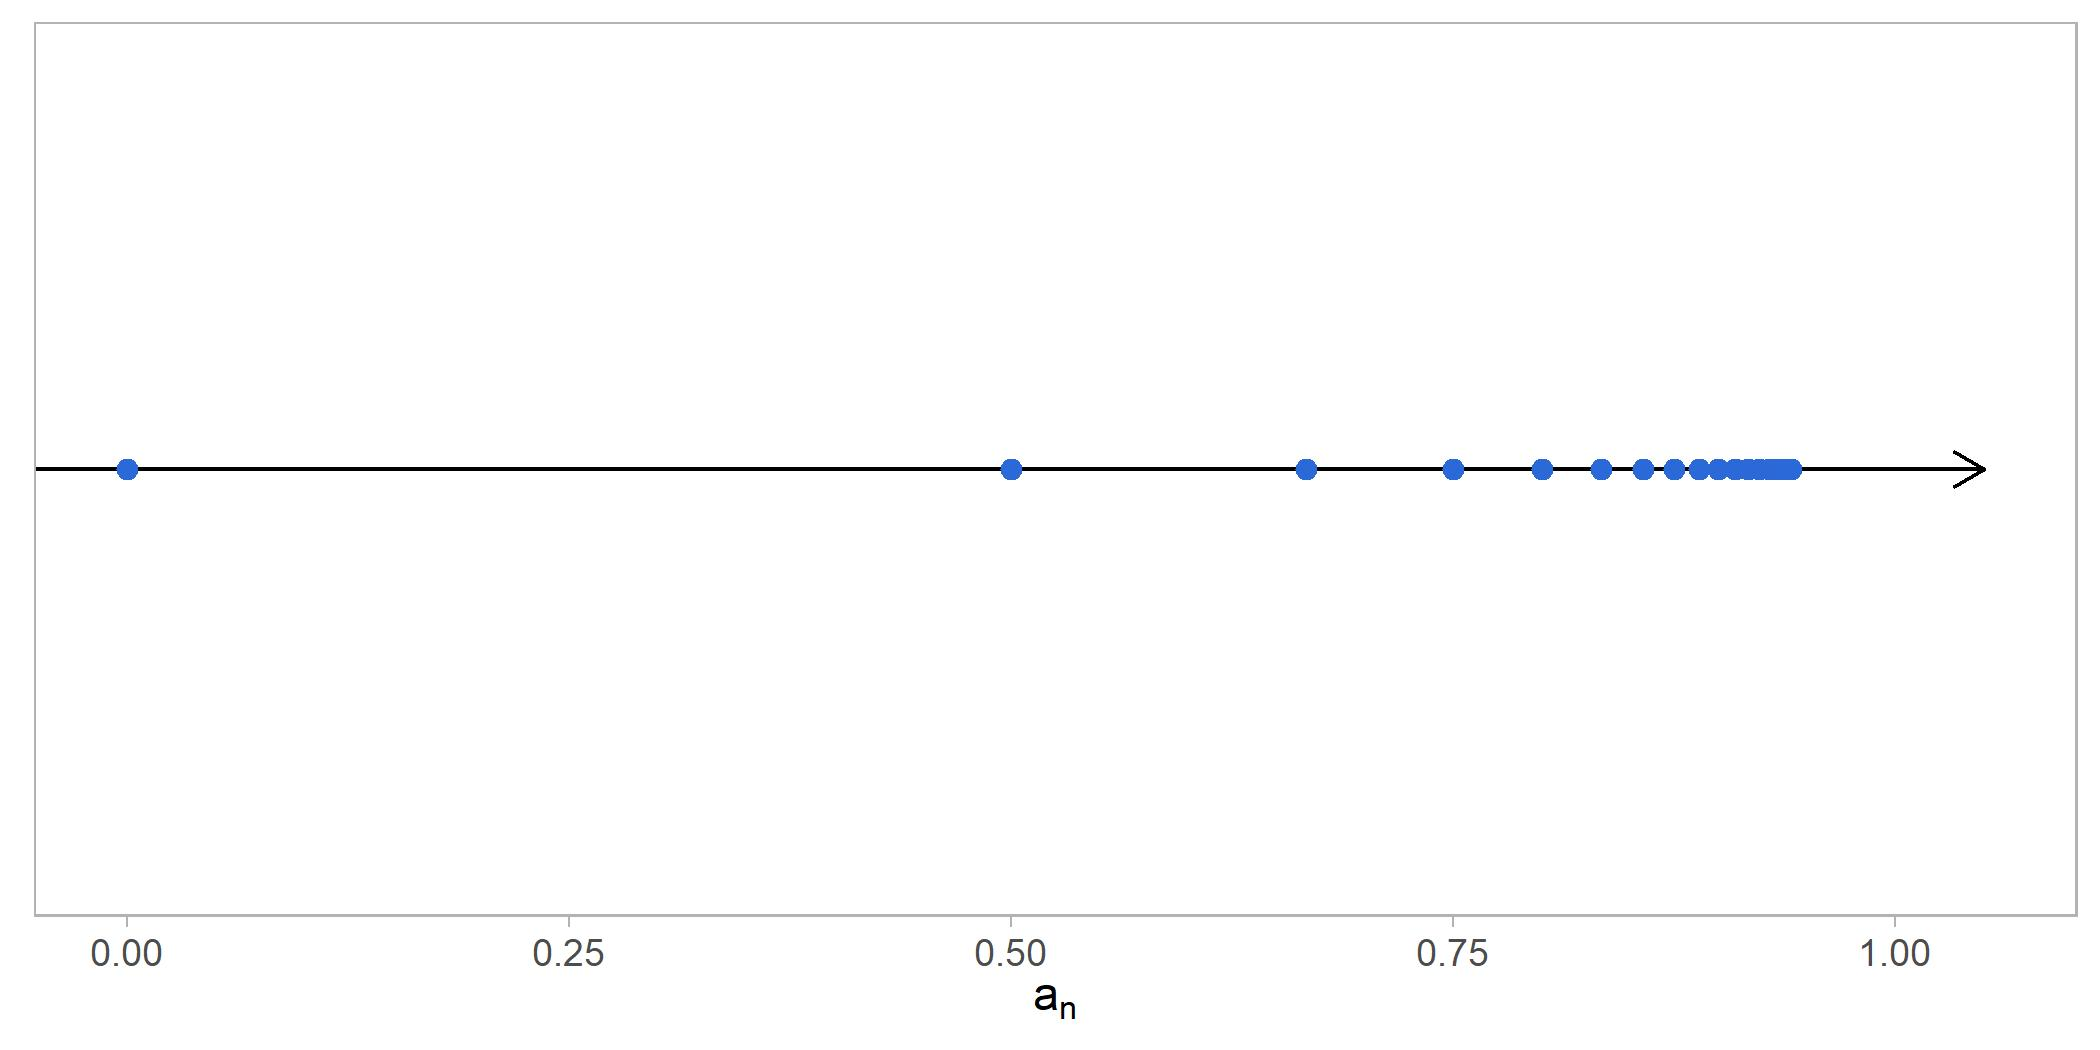
\includegraphics[scale=0.7]{rect-line-plot.jpg}
\end{figure}

\newpage

Mientras que la representación gráfica de $\{a_{n}\}$ en el plano $xy$ es la siguiente.

\begin{figure}[hbt!]
\centering
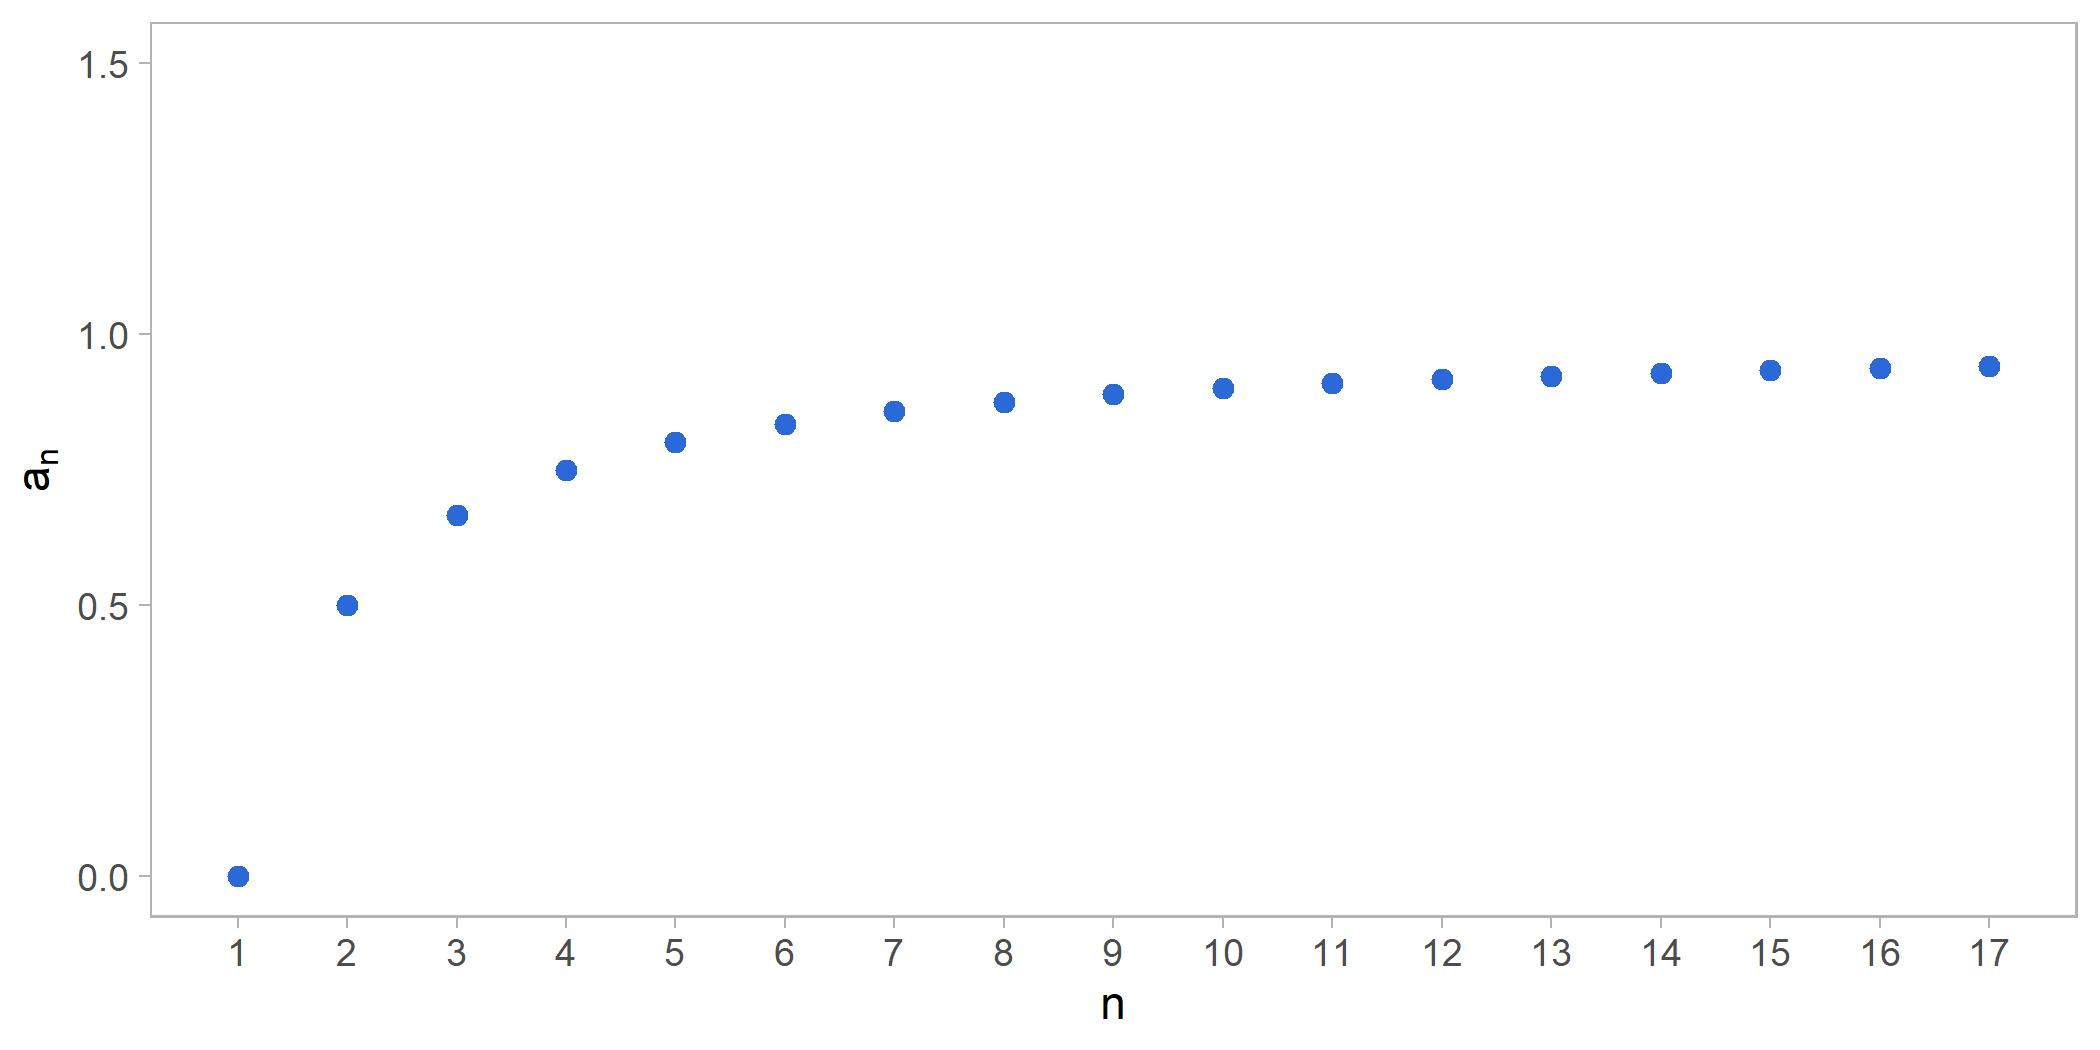
\includegraphics[scale=0.7]{xy-plane-plot.jpg}
\end{figure}

En cuanto a las dos gráficas vistas de $\{a_{n}\}$, \textbf{es más habitual su representación en el plano $xy$}. Como se aprecia en la imagen de arriba, ilustra mejor el comportamiento de la sucesión, lo que es clave para realizar distintos análisis sobre ella.


\section{El límite de una sucesión.}

Es posible evaluar en una sucesión infinita $\{a_{n}\}$ si, a medida que $n \to \infty$, sus términos resultantes $a_{n}$ son cada vez más cercanos (o no) a un número finito $L$. Es decir,
\[
  \lim_{n \to \infty} a_{n} = L
\]
donde $L$ es el \textbf{límite de la sucesión} de $\{a_{n}\}$.

Si $a_{n} \to L$ a medida que $n \to \infty$, se dice que la sucesión $\{a_{n}\}$ es \textbf{convergente}. En cambio, cuando no se aproxima a dicho valor, se concluye que es \textbf{divergente}.

Una \textbf{definición más precisa} señala que $\{a_{n}\}$ \textbf{converge} a un valor $L$ mientras $n \to \infty$ si, para todo número $\epsilon > 0$ hay un correspondiente $N \in \mathbb{Z}$ tal que, cuando $n > N$,
\[
  |a_{n} - L| < \epsilon
\]
$\epsilon$ es un número positivo cualquiera y $N$ es el índice de un término específico de $\{a_{n}\}$. Lo que indica esta definición, es que podemos confirmar que esta sucesión es convergente si la distancia entre cada término superior a $a_{N}$  (e.g, $a_{N + 1}$) y su límite $L$ es menor a $\epsilon$.

Otra manera de explicar esta definición, es estableciendo un intervalo $(L - \epsilon, \ L + \epsilon)$. Se verifica que $\{a_{n}\}$ es convergente si todos sus términos posteriores a $a_{N}$ están adentro de dicho rango.

Por ejemplo, la siguiente sucesión es convergente.
\[
  \lim_{n \to \infty} \left\{(-1)^{n + 1} \left(\frac{1}{n}\right)\right\} = 0
\]
Si se establece que $\epsilon = 0.4$, todas las entradas posteriores, digamos, al segundo término ($N = 2$) están eventualmente adentro de $(0 - 0.4, \ 0 + 0.4)$ y cada vez más cercanos a $L = 0$ ya que la sucesión \textbf{converge} a ese valor, como se observa en la siguiente gráfica.

\begin{figure}[hbt!]
\centering
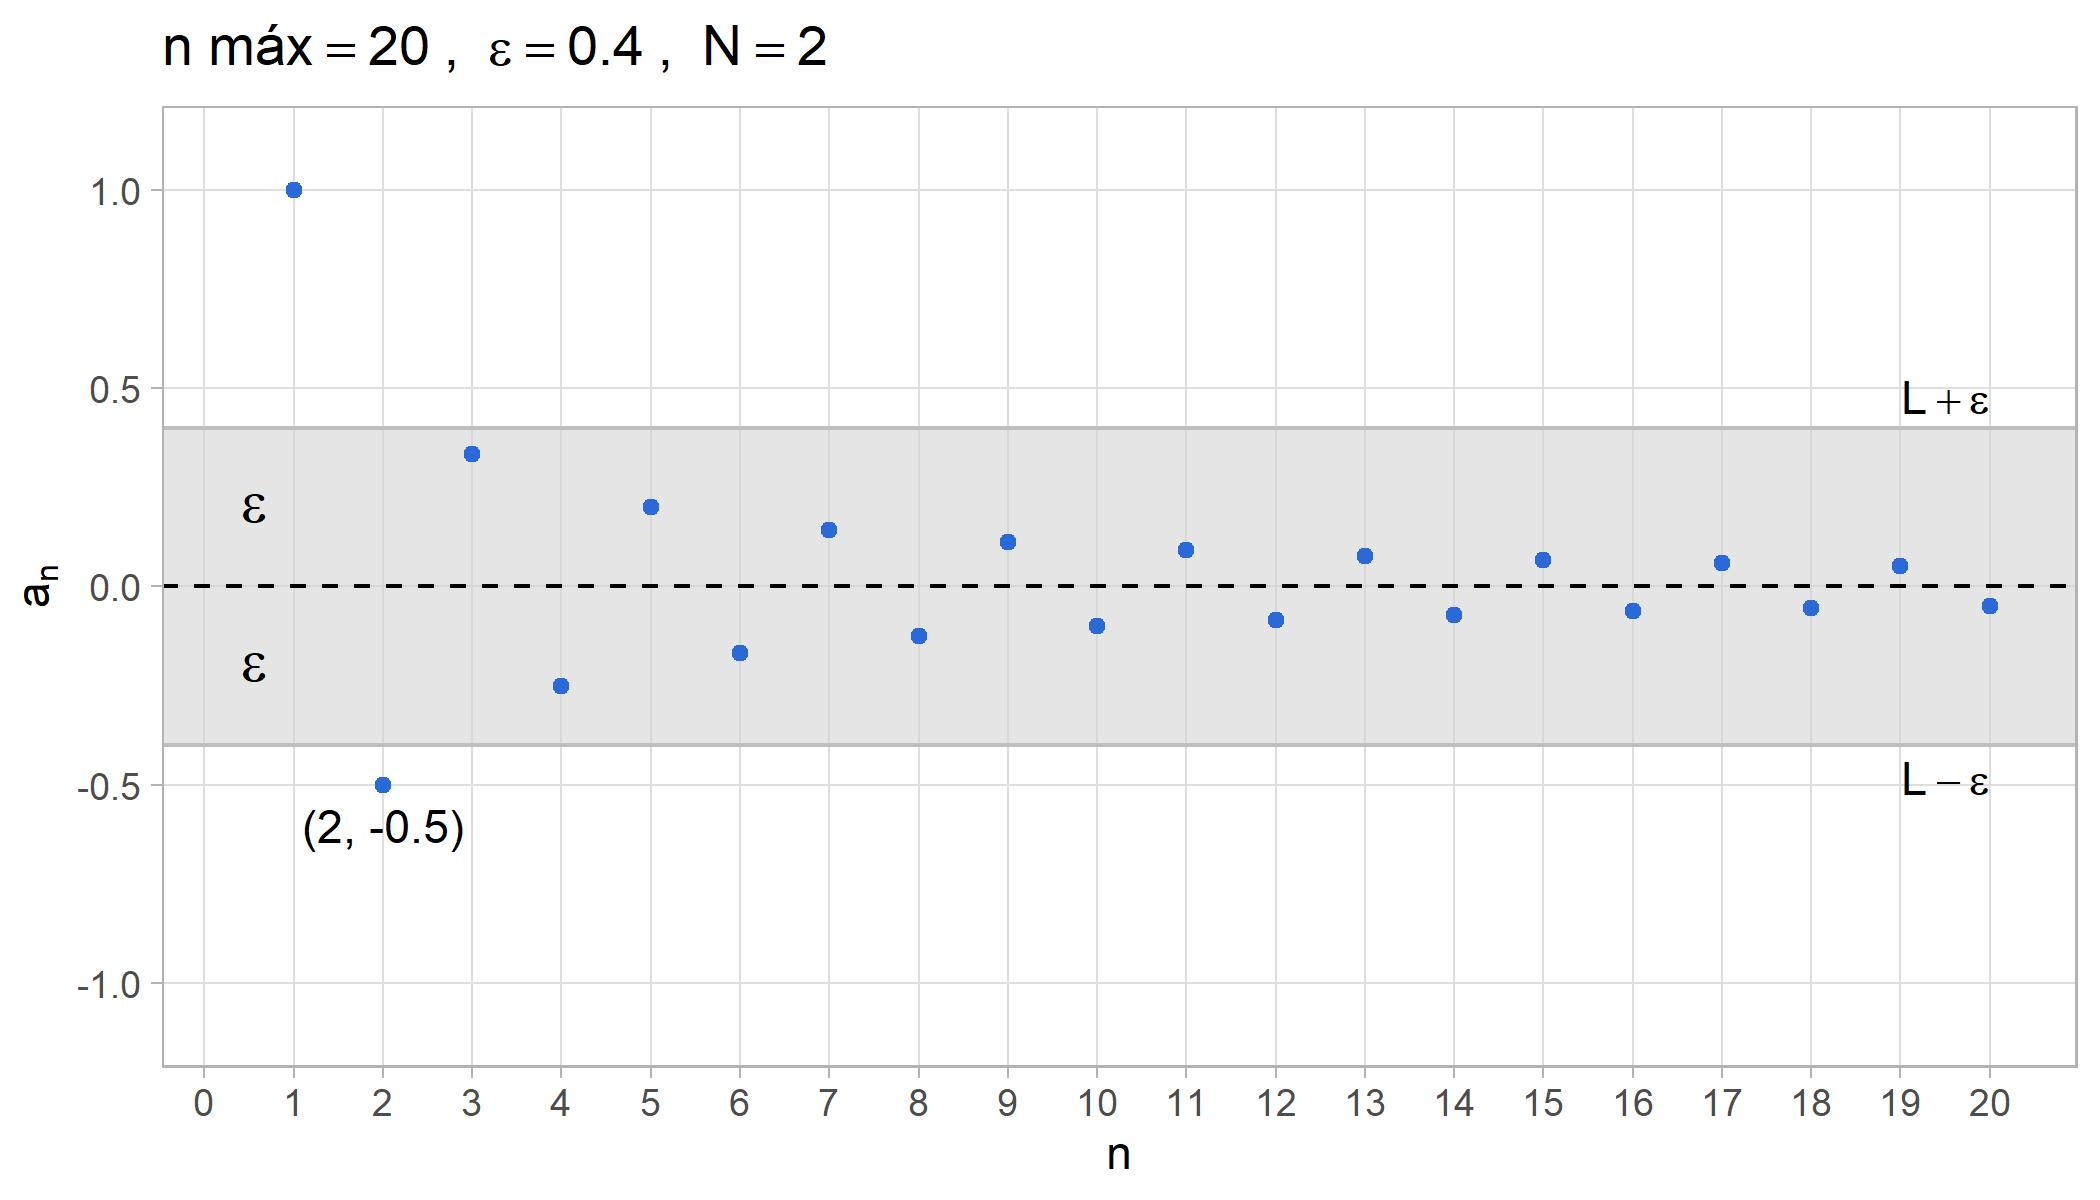
\includegraphics[scale=0.7]{limit-seq-01.jpg}
\end{figure}

Incluso se cumple si definimos que $\epsilon = 0.15$.

\begin{figure}[hbt!]
\centering
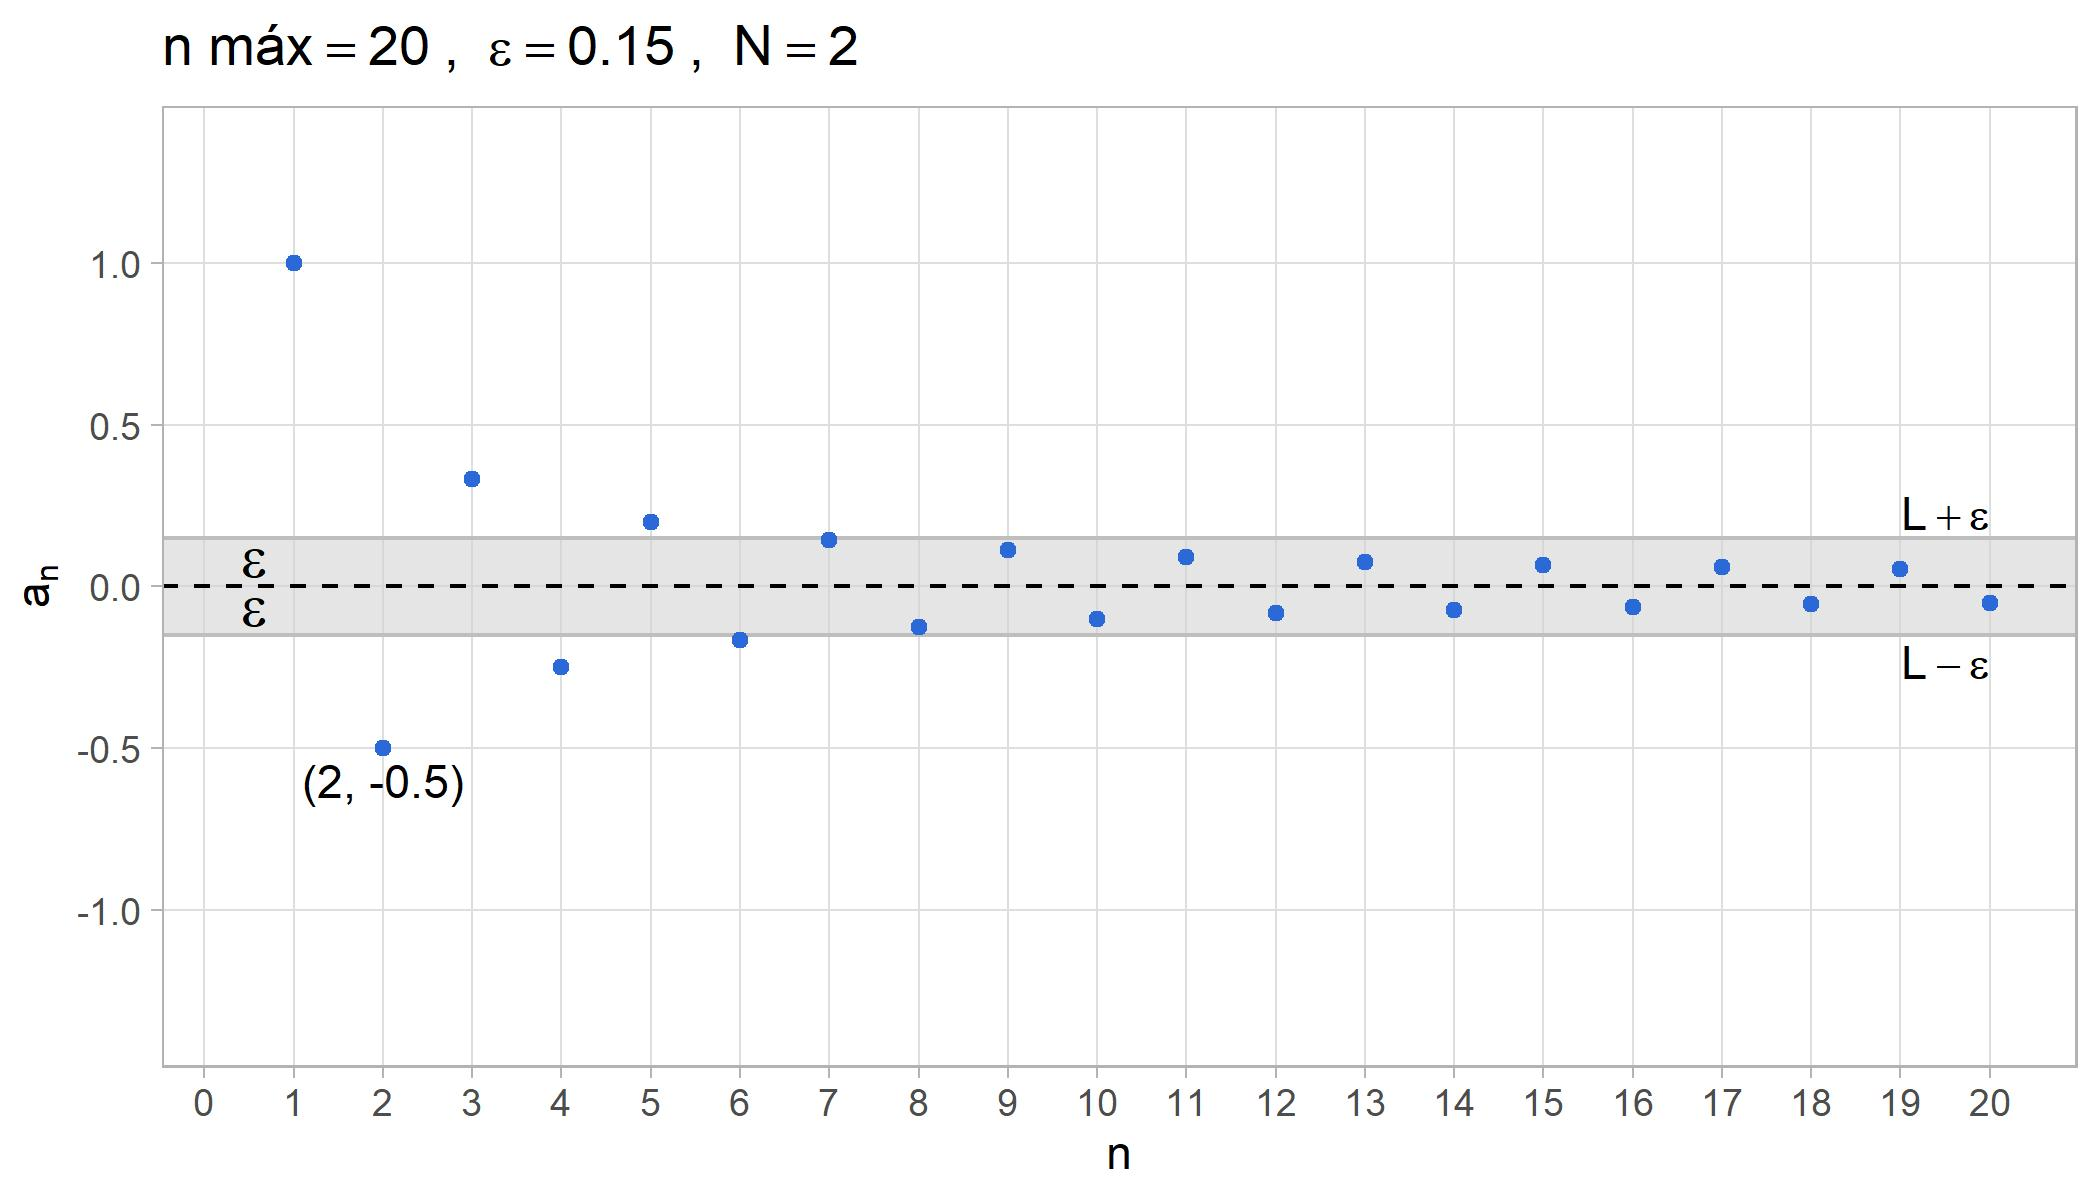
\includegraphics[scale=0.7]{limit-seq-02.jpg}
\end{figure}

En cuanto a las sucesiones \textbf{divergentes}, en general pueden serlo por dos motivos:

\begin{enumerate}
\item $\lim_{n \to \infty} a_{n} = \pm \infty$.
\item $\lim_{n \to \infty} a_{n} \neq \pm \infty$, pero sus términos no se aproximan a un valor determinado.
\end{enumerate}

Un ejemplo del punto 2 es $\{a_{n}\} = (-1)^{n}$. Para cualquier $n \geq 0$, sus términos siempre serán $\pm 1$ y esto no cambia mientras $n \to \infty$, es por ello que se concluye que es \textbf{divergente} porque si bien en su límite no se aproxima al $\pm \infty$, tampoco lo hace a un valor finito $L$.

\begin{table}[hbt!]
\centering

\begin{tabular}{c | c c c c c}
$n$ & $1$ & $2$ & $3$ & $4$ & $\ldots$ \\
\hline
$a_{n}$ & $-1$ & $1$ & $-1$ & $1$ & $\ldots$
\end{tabular}

\end{table}

\subsection{Cálculo del límite de una sucesión.}

Las reglas para calcular el límite de una sucesión, en general, son las mismas a las usadas cuando realizamos dicha evaluación en una función.

Sean $\{a_{n}\}$ y $\{b_{n}\}$ dos sucesiones, mientras que $A$ y $B$ son números reales. Si se cumple con que:
\[
  \lim_{n \to \infty} a_{n} = A \qquad \text{y} \qquad \lim_{n \to \infty} b_{n} = B,
\]
entonces podemos usar las siguientes reglas con sus límites:
\begin{align*}
& 1. \ \text{Regla de la suma}               &\lim_{n \to \infty} (a_{n} + b_{n}) = A + B \\
& 2. \ \text{Regla de la diferencia}         &\lim_{n \to \infty} (a_{n} - b_{n}) = A - B \\
& 3. \ \text{Regla del múltiplo constante}   &\lim_{n \to \infty} (k \cdot b_{n}) = k \cdot B \ (k = \text{cte}) \\
& 4. \ \text{Regla del producto}             &\lim_{n \to \infty} (a_{n} \cdot b_{n}) = A \cdot B \\
& 5. \ \text{Regla del cociente}             &\lim_{n \to \infty} \frac{a_{n}}{b_{n}} = \frac{A}{B} \iff B \neq 0
\end{align*}
Además, si una sucesión es descrita como una fracción con polinomios en su denominador y/o numerador, también es posible simplificarla a partir del término de mayor grado como lo hemos hecho al trabajar con funciones.

\subsection{Regla de L'Hôpital en sucesiones.}

Al calcular el límite de una sucesión podría surgir la idea de resolverla usando la regla de L'Hôpital debido a que, en principio, obtuvimos una forma indeterminada. El problema es que solo se aplica a funciones que, además, son derivables\footnote{Revisar apuntes de la Clase 35 para mayor detalle.}. No obstante, de igual modo existe una relación entre los límites de una función y de una sucesión que nos permite usarla.

Sean $f(x)$ una función definida en $x \geq n_{0}$ y $\{a_{n}\}$ una sucesión de números reales tal que $a_{n} = f(n)$ para todo $n \geq n_{0}$. Si, bajo este contexto, se cumple que:
\[
  \lim_{x \to \infty} f(x) = L \qquad \text{entonces} \qquad \lim_{n \to \infty} a_{n} = L
\]
Lo que nos dice esta relación es que, bajo dichas condiciones, \textbf{el comportamiento de} $\{a_{n}\}$ \textbf{se asemeja al de} $f(x)$. Por lo tanto, si calculamos el límite de $\{a_{n}\}$ y obtenemos una forma indeterminada, podemos trabajarla como $f(x)$ para aplicar la regla de L'Hôpital.

\textbf{Ejemplo.} Evalúe si la siguiente sucesión es convergente o divergente.
\[
  \{a_{n}\} = \left(\frac{n + 1}{n - 1}\right)^{n}
\]
\textbf{Solución.} Comencemos evaluando el límite de esta sucesión.
\[
  \lim_{n \to \infty} \left(\frac{n + 1}{n - 1}\right)^{n} = \lim_{n \to \infty} \left(\frac{1 + (1/n)}{1 - (1/n)}\right)^{n}
                                                           = \left(\frac{1 + 0}{1 - 0}\right)^{\infty}
                                                           = 1^{\infty}
\]
Veamos si podemos usar la regla de L'Hôpital en este límite. Primero, tratemos de llevarla a la forma indeterminada $0/0$ usando el siguiente procedimiento estudiado en la Clase 35.
\[
\lim_{n \to \infty} \left(\frac{n + 1}{n - 1}\right)^{n} = \lim_{n \to \infty} \exp\left(\ln\left[\left(\frac{n + 1}{n - 1}\right)^{n}\right]\right)
                                                         = \lim_{n \to \infty} \exp\left(n \cdot \ln\left[\frac{n + 1}{n - 1}\right]\right)
\]
Esto nos permite calcular el límite del exponente de $\exp()$.
\[
\lim_{n \to \infty} \left(\frac{n + 1}{n - 1}\right)^{n} = \exp\left(\lim_{n \to \infty} n \cdot \ln\left[\frac{n + 1}{n - 1}\right]\right)
\]
donde
\[
\lim_{n \to \infty} n \cdot \ln\left[\frac{n + 1}{n - 1}\right] = \lim_{n \to \infty} \frac{\ln[(n + 1)/(n - 1)]}{(1/n)}
                                                                = \frac{\ln[1]}{0}
                                                                = \frac{0}{0}
\]
Para todo $n \geq 2$, con $n \in \mathbb{Z}$, es posible observar que las sucesiones $\ln[(n + 1)/(n - 1)]$ y $1/n$ se comportan de manera semejante a las funciones $\ln[(x + 1)/(x - 1)]$ y $1/x$, ya que estas últimas están definidas para dicho valor. Por lo tanto, podemos utilizar la regla de L'Hôpital en el límite que calculamos arriba.

\begin{align*}
\lim_{n \to \infty} n \cdot \ln\left[\frac{n + 1}{n - 1}\right] &= \lim_{n \to \infty} \frac{\ln[(n + 1)/(n - 1)]}{(1/n)} \\
                                                                &= \lim_{n \to \infty} \frac{((n - 1)/(n + 1)) \cdot (((n - 1) - (n + 1))/(n - 1)^{2})}{-1/n^{2}} \\
                                                                &= \lim_{n \to \infty} \frac{(-2)/(n^{2} - 1)}{-1/n^{2}} \\
                                                                &= \lim_{n \to \infty} \frac{2n^{2}}{n^{2} - 1} \\
                                                                &= \lim_{n \to \infty} \frac{2}{1 - (1/n^{2})} \\
                                                                &= 2
\end{align*}
Por lo tanto,
\[
  \lim_{n \to \infty} \left(\frac{n + 1}{n - 1}\right)^{n} = \exp\left(\lim_{n \to \infty} n \cdot \ln\left[\frac{n + 1}{n - 1}\right]\right)
                                                           = \exp(2)
                                                           \approx 7.389
\]
Es decir, podemos concluir que la sucesión de este ejemplo es \textbf{convergente}, ya que $a_{n} \to \exp(2)$ a medida que $n \to \infty$ como se ve en su gráfica.

\begin{figure}[hbt!]
\centering
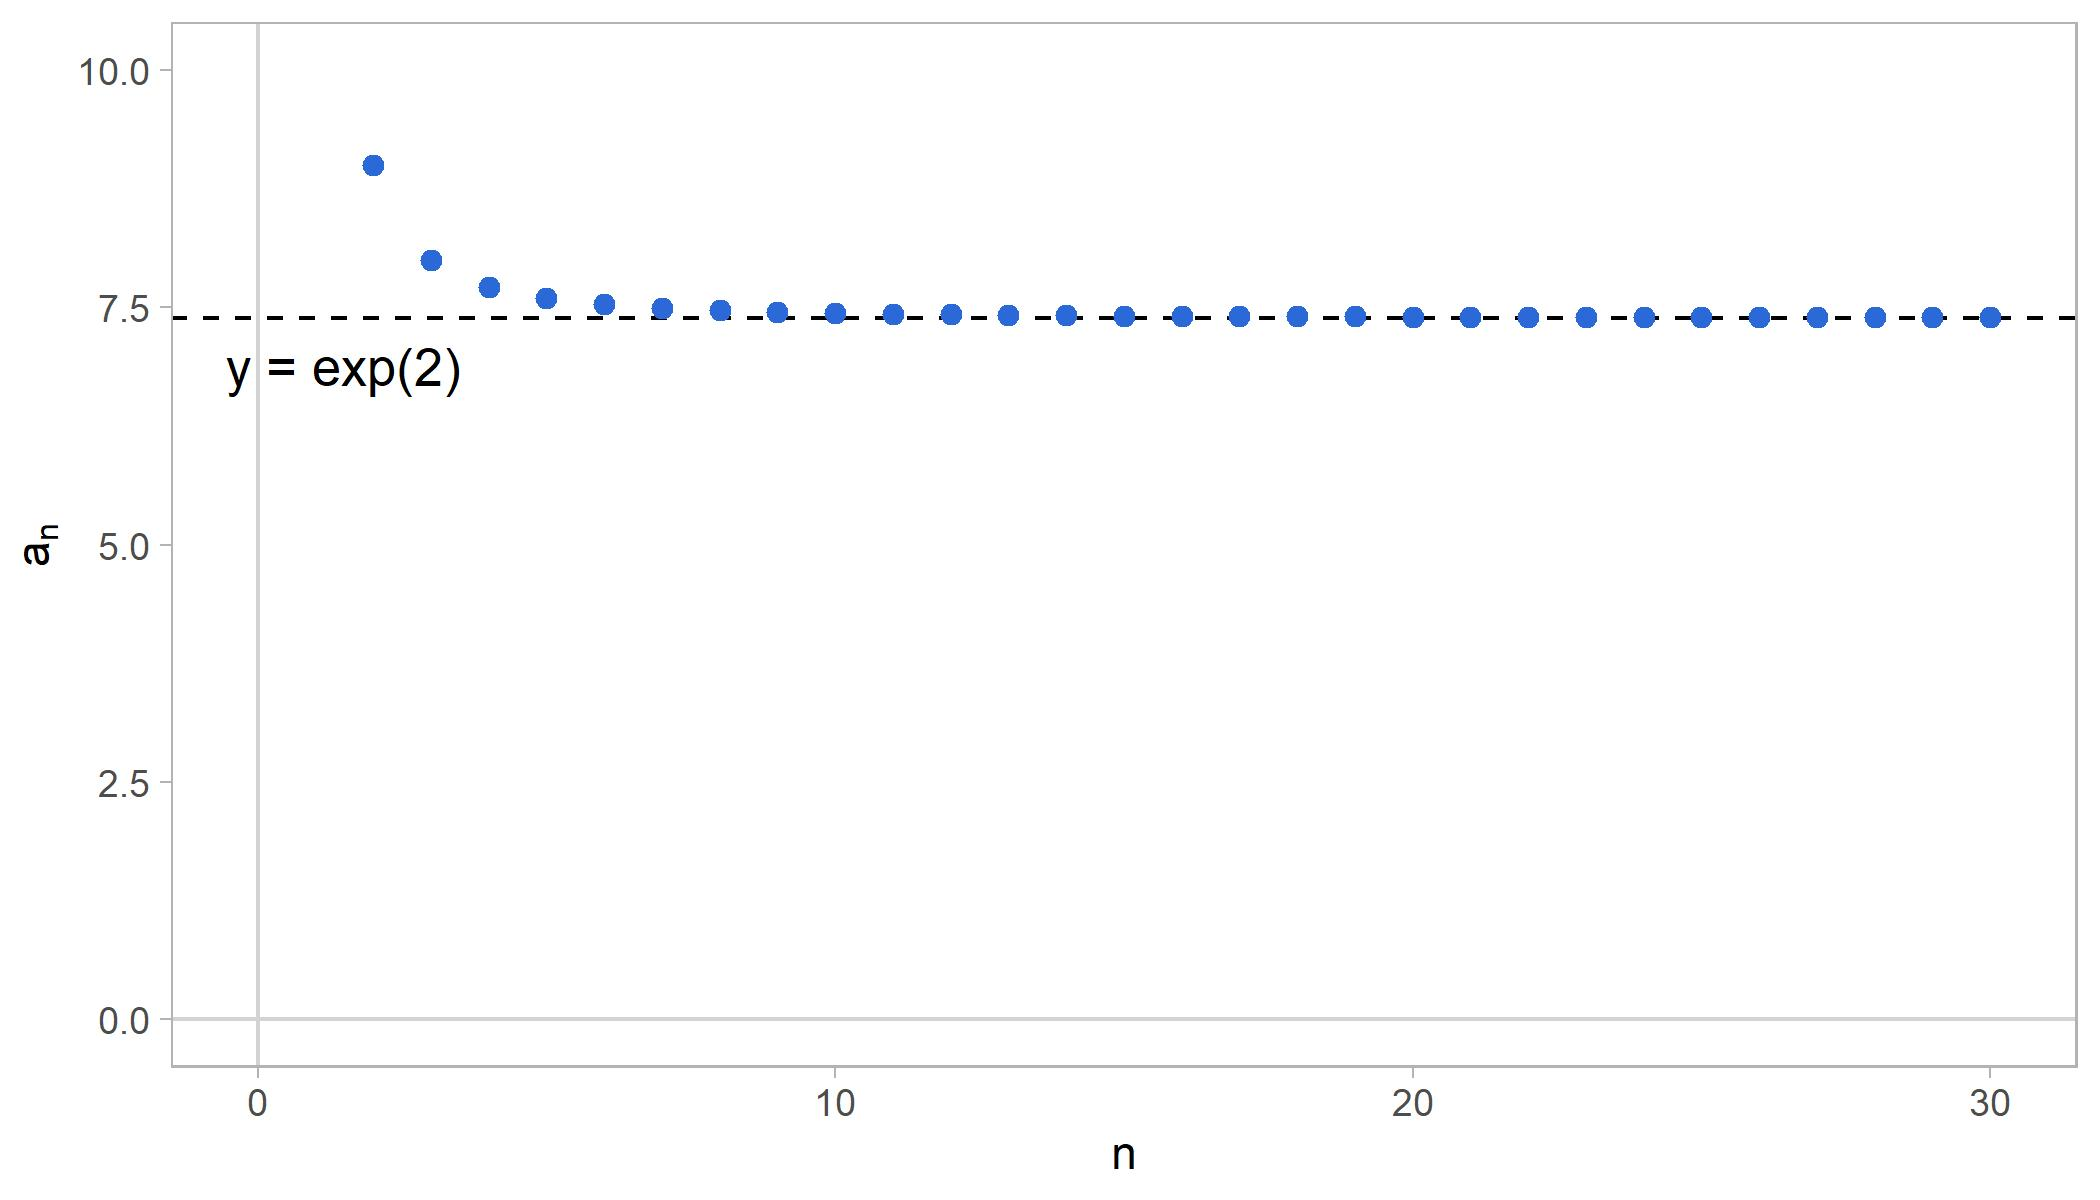
\includegraphics[scale=0.7]{limit-lhopital-example.jpg}
\end{figure}


\section{Evaluando la convergencia de una sucesión.}

Hasta ahora sabemos evaluar la convergencia de una sucesión a partir de la existencia de su límite. No obstante, también es posible determinar aquello según si está \textbf{acotada} y si es \textbf{monótona}. Dichos conceptos los veremos a continuación.

\subsection{Sucesión acotada.}

Es posible que una sucesión esté limitada a valores específicos. Es decir, que sus términos no tomen valores mayores y/o menores a ellos. En dichos casos se señala que está acotada por arriba, por abajo o por ambos lados.

Formalmante, una sucesión $\{a_{n}\}$ está \textbf{acotada por arriba} si existe un número $M$ tal que:
\[
  a_{n} \leq M; \quad \forall n \in \mathbb{Z}
\]
En dicho caso se dice que $M$ es una \textbf{cota superior} de $\{a_{n}\}$. Si no hay otro número menor a $M$ que cumpla dicha característica, se concluye que es una \textbf{mínima cota superior} de la sucesión.

Por otra parte, la sucesión $\{a_{n}\}$ está \textbf{acotada por abajo} si existe un número $m$ tal que:
\[
  a_{n} \geq m; \quad \forall n \in \mathbb{Z}
\]
En este caso, $m$ es la \textbf{cota inferior} de $\{a_{n}\}$ y si no hay otro número menor que $m$ que también lo sea, se señala que $m$ es la \textbf{máxima cota inferior} de $\{a_{n}\}$.

Así, una \textbf{sucesión acotada} es aquella que está \textbf{acotada tanto por arriba como por abajo}.

Las sucesiones convergentes se caracterizan por ser acotadas, pero \textbf{no todas las sucesiones acotadas son convergentes}. Un caso es el de la sucesión $\{a_{n}\} = (-1)^{n}$ vista anteriormente (página 6). Como vemos en su gráfica, está acotada a $\pm 1$, pero aun así no es convergente.

\begin{figure}[hbt!]
\centering
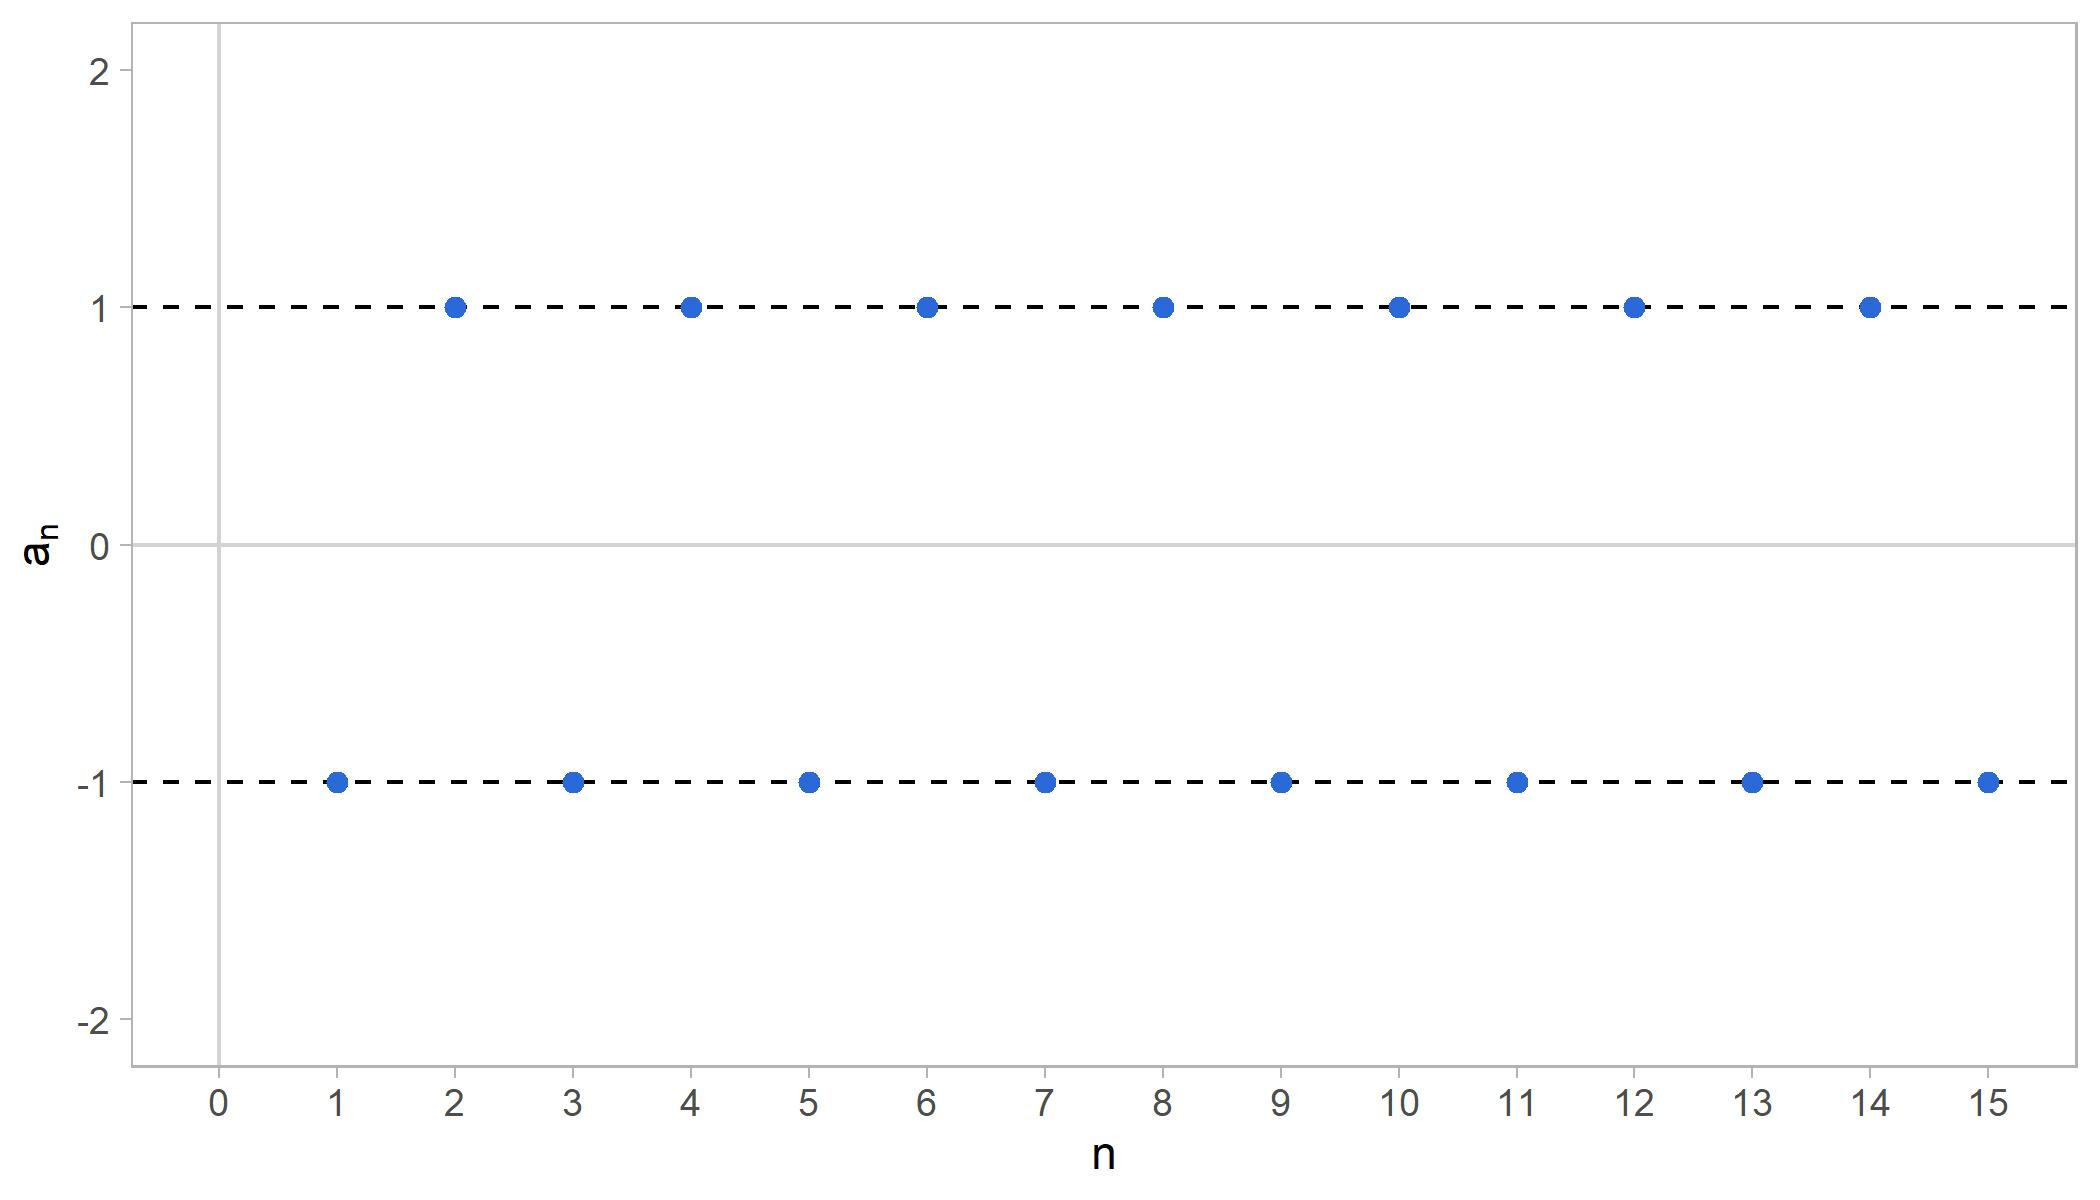
\includegraphics[scale = 0.7]{bounded-not-convergent-plot.jpg}
\end{figure}

Por lo tanto, es necesario un criterio adicional para determinar que una sucesión sea convergente y éste corresponde a que sea monótona.

\subsection{Sucesión monótona.}

Una sucesión $\{a_{n}\}$ puede ser no-decreciente, que es cuando sus términos
\[
  a_{1} \leq a_{2} \leq a_{3} \leq \cdots \leq a_{n} \leq \cdots
\]
o no-creciente, donde sus términos
\[
  a_{1} \geq a_{2} \geq a_{3} \geq \cdots \geq a_{n} \geq \cdots
\]
Se define que una sucesión es \textbf{monótona} cuando \textbf{es no-decreciente o no-creciente}.

Una \textbf{sucesión monótona} va a estar acotada por al menos un lado, pero no siempre en los dos. Este último caso significa que sus términos crecen al $\pm \infty$, de manera que \textbf{debe ser acotada para ser convergente}. Esto nos lleva al siguiente teorema.

\subsection{Teorema de la sucesión monótona.}

El \textbf{teorema de la sucesión monótona} señala que si una sucesión $\{a_{n}\}$ es \textbf{acotada y monótona}, entonces \textbf{es convergente}.

Como se señaló antes, una sucesión monótona siempre estará acotada por un lado y debe estarlo por el otro para que sea convergente. Lo que formaliza este teorema es que, en dicho caso, el límite $L$ de $\{a_{n}\}$ será su mínima cota superior o su máxima cota inferior.

\textbf{Demostración}. Sea $\{a_{n}\}$ una sucesión no-decreciente con una cota superior $M$.
\[
  a_{1} \leq a_{2} \leq \cdots \leq a_{n} \leq \cdots \leq M
\]
Por la existencia de $M$, se puede utilizar el \textbf{Axioma de completitud} o \textbf{del supremo} para esta demostración.

Digamos que un conjunto no vacío $S \subseteq \mathbb{R}$. El \textbf{axioma de completitud} señala que si $S$ tiene una \textbf{cota superior}, se puede asegurar que también tiene una \textbf{cota mínima superior}.

En este caso, podemos establecer que $S = \{a_{n} \ | \ n \geq 1\}$. Como $\{a_{n}\}$ tiene una cota superior $M$, por el axioma de completitud es válido señalar que también tiene una cota mínima superior que denotaremos como $L$, donde $L \leq M$. Es decir,
\[
  a_{1} \leq a_{2} \leq \cdots \leq a_{n} \leq \cdots \leq L
\]
También se expresa como $\sup\{a_{n}\} = L$, donde $\sup$ es el \textbf{supremo} (\textit{supremum} en inglés) de $\{a_{n}\}$.

Ahora, para todo $\epsilon > 0$ se cumple que $L - \epsilon < L$, es decir $L - \epsilon$ no es una cota superior de $\{a_{n}\}$ al ser menor a su cota mínima superior. Esto implica que al menos un término $a_{N}$ de esta sucesión, con $N \in \mathbb{Z}$ y $N \geq 0$, será mayor a dicha diferencia.
\[
  a_{N} > L - \epsilon
\]
Por otra parte, para todo $n > N$, $a_{n} \geq a_{N}$ debido a que $\{a_{n}\}$ es no-decreciente, lo que también significa que $a_{n} > L - \epsilon$. A partir de lo que se ha señalado en esta demostración, es posible afirmar que:
\[
  L - \epsilon < a_{N} \leq a_{n} \leq L < L + \epsilon; \quad \forall n > N
\]
De la desigualdad compuesta de arriba es posible observar lo siguiente:
\[
  L - \epsilon < a_{n} < L + \epsilon
\]
Lo cual es lo mismo a:
\[
  - \epsilon < a_{n} - L < \epsilon
\]
Si tomamos el \textbf{valor absoluto} de esta desigualdad compuesta, por la propiedad de este tipo en particular se concluye que
\[
  |a_{n} - L| < \epsilon
\]
Esta es la desigualdad que nos indica que, para todo $\epsilon > 0$ y $n > N$, la sucesión $\{a_{n}\}$ es \textbf{convergente} (página 4) que, en este caso, lo hace a $L$. Por lo tanto, \textbf{ha quedando demostrado este teorema}.

Es decir, una sucesión $\{a_{n}\}$ no-decreciente es convergente sí y solo sí está acotada. En ese caso, lo hace a su cota mínima superior $L$ la que, además, corresponde a su \textbf{límite al infinito}.
\[
  \lim_{n \to \infty} a_{n} = \sup\{a_{n}\} = L
\]
Esta demostración también es aplicable en sucesiones acotadas no-crecientes.

\end{document}
